\documentclass[a4paper,14pt]{extreport} % формат документа

\usepackage{amsmath}
\usepackage{cmap} % поиск в ПДФ
\usepackage[T2A]{fontenc} % кодировка
\usepackage[utf8]{inputenc} % кодировка исходного текста
\usepackage[english,russian]{babel} % локализация и переносы
\usepackage[left = 2cm, right = 1cm, top = 2cm, bottom = 2 cm]{geometry} % поля
\usepackage{listings}
\usepackage{graphicx} % для вставки рисунков
\usepackage{amsmath}
\usepackage{float}
\usepackage{multirow}
\graphicspath{{pictures/}}
\usepackage{amsfonts}
\DeclareGraphicsExtensions{.pdf,.png,.jpg}
\newcommand{\anonsection}[1]{\section*{#1}\addcontentsline{toc}{section}{#1}}

\renewcommand{\thesection}{\arabic{section}}

\lstset{ %
	language=Matlab,                % Язык программирования 
	numbers=left,                   % С какой стороны нумеровать          
	frame=single,                    % Добавить рамку
	escapebegin=\begin{russian}\commentfont,
    escapeend=\end{russian},
    basicstyle=\small,
    literate={Ö}{{\"O}}1
    {Ä}{{\"A}}1
    {Ü}{{\"U}}1
    {ß}{{\ss}}1
    {ü}{{\"u}}1
    {ä}{{\"a}}1
    {ö}{{\"o}}1
    {~}{{\textasciitilde}}1
    {а}{{\selectfont\char224}}1
    {б}{{\selectfont\char225}}1
    {в}{{\selectfont\char226}}1
    {г}{{\selectfont\char227}}1
    {д}{{\selectfont\char228}}1
    {е}{{\selectfont\char229}}1
    {ё}{{\"e}}1
    {ж}{{\selectfont\char230}}1
    {з}{{\selectfont\char231}}1
    {и}{{\selectfont\char232}}1
    {й}{{\selectfont\char233}}1
    {к}{{\selectfont\char234}}1
    {л}{{\selectfont\char235}}1
    {м}{{\selectfont\char236}}1
    {н}{{\selectfont\char237}}1
    {о}{{\selectfont\char238}}1
    {п}{{\selectfont\char239}}1
    {р}{{\selectfont\char240}}1
    {с}{{\selectfont\char241}}1
    {т}{{\selectfont\char242}}1
    {у}{{\selectfont\char243}}1
    {ф}{{\selectfont\char244}}1
    {х}{{\selectfont\char245}}1
    {ц}{{\selectfont\char246}}1
    {ч}{{\selectfont\char247}}1
    {ш}{{\selectfont\char248}}1
    {щ}{{\selectfont\char249}}1
    {ъ}{{\selectfont\char250}}1
    {ы}{{\selectfont\char251}}1
    {ь}{{\selectfont\char252}}1
    {э}{{\selectfont\char253}}1
    {ю}{{\selectfont\char254}}1
    {я}{{\selectfont\char255}}1
    {А}{{\selectfont\char192}}1
    {Б}{{\selectfont\char193}}1
    {В}{{\selectfont\char194}}1
    {Г}{{\selectfont\char195}}1
    {Д}{{\selectfont\char196}}1
    {Е}{{\selectfont\char197}}1
    {Ё}{{\"E}}1
    {Ж}{{\selectfont\char198}}1
    {З}{{\selectfont\char199}}1
    {И}{{\selectfont\char200}}1
    {Й}{{\selectfont\char201}}1
    {К}{{\selectfont\char202}}1
    {Л}{{\selectfont\char203}}1
    {М}{{\selectfont\char204}}1
    {Н}{{\selectfont\char205}}1
    {О}{{\selectfont\char206}}1
    {П}{{\selectfont\char207}}1
    {Р}{{\selectfont\char208}}1
    {С}{{\selectfont\char209}}1
    {Т}{{\selectfont\char210}}1
    {У}{{\selectfont\char211}}1
    {Ф}{{\selectfont\char212}}1
    {Х}{{\selectfont\char213}}1
    {Ц}{{\selectfont\char214}}1
    {Ч}{{\selectfont\char215}}1
    {Ш}{{\selectfont\char216}}1
    {Щ}{{\selectfont\char217}}1
    {Ъ}{{\selectfont\char218}}1
    {Ы}{{\selectfont\char219}}1
    {Ь}{{\selectfont\char220}}1
    {Э}{{\selectfont\char221}}1
    {Ю}{{\selectfont\char222}}1
    {Я}{{\selectfont\char223}}1
    {і}{{\selectfont\char105}}1
    {ї}{{\selectfont\char168}}1
    {є}{{\selectfont\char185}}1
    {ґ}{{\selectfont\char160}}1
    {І}{{\selectfont\char73}}1
    {Ї}{{\selectfont\char136}}1
    {Є}{{\selectfont\char153}}1
    {Ґ}{{\selectfont\char128}}1
}

\begin{document}
\begin{titlepage}

    \begin{table}[H]
        \centering
        \footnotesize
        \begin{tabular}{cc}
            \multirow{8}{*}{
\includegraphics[scale=0.35]{bmstu.jpg}}
            & \\
            & \\
            & \textbf{Министерство науки и высшего образования Российской Федерации} \\
            & \textbf{Федеральное государственное бюджетное образовательное учреждение} \\
            & \textbf{высшего образования} \\
            & \textbf{<<Московский государственный технический} \\
            & \textbf{университет имени Н.Э. Баумана>>} \\
            & \textbf{(МГТУ им. Н.Э. Баумана)} \\
        \end{tabular}
    \end{table}

    \vspace{-2.5cm}

    \begin{flushleft}
        \rule[-1cm]{\textwidth}{3pt}
        \rule{\textwidth}{1pt}
    \end{flushleft}

    \begin{flushleft}
        \small
        ФАКУЛЬТЕТ
        \underline{<<Информатика и системы управления>>\ \ \ \ \ \ \ 
        \ \ \ \ \ \ \ \ \ \ \ \ \ \ \ \ \ \ \ \ \ \ \ \ \ \ \ \ \ \ \ 
    \ \ \ \ \ \ \ \ \ \ \ \ \ \ \ } \\
        КАФЕДРА
        \underline{<<Программное обеспечение ЭВМ и
        информационные технологии>>
        \ \ \ \ \ \ \ \ \ \ \ \ \ \ \ \ \ \ \ \ }
    \end{flushleft}

    \vspace{2cm}

    \begin{center}
        \textbf{Лабораторная работа № 1} \\
        \vspace{0.5cm}
    \end{center}

    \vspace{4cm}

    \begin{flushleft}
        \begin{tabular}{ll}
            \textbf{Дисциплина} & Математическая статистика.  \\
            \textbf{Тема} & Гистограмма и эмпирическая функция распределения.   \\
            \\
            \textbf{Студент} & Сиденко А.Г. \\
            \textbf{Группа} & ИУ7-63Б \\
            \textbf{Оценка (баллы)} & \\
            \textbf{Преподаватель} & Власов П.А.   \\
        \end{tabular}
    \end{flushleft}

    \vspace{4cm}

   \begin{center}
        Москва, 2020 г.
    \end{center}

\end{titlepage}

\section{Формулы для вычисления величин}

$$\vec X=(X_1, ..., X_n)$$

\begin{enumerate}
\item \textbf{Максимальное значение выборки}
$$M_{\max} = \max\{X_1, .., X_n\}$$
\item \textbf{Минимальное значение выборки}
$$M_{\min} = \min\{X_1, .., X_n\}$$
\item \textbf{Размах выборки}
$$R = M_{\max} - M_{\min}$$
\item \textbf{Выборочное среднее (математическое ожидание)}
$$\hat \mu(\vec X) = \frac{1}{n} \sum_{i=1}^n X_i$$
\item \textbf{Состоятельная оценка дисперсии}
$$S^2 (\vec X) = \frac{1}{n-1} \sum_{i=1}^n (X_i - \overline X)^2$$

где $ \overline{X} = \hat m $
\end{enumerate}

\section{Определение эмпирической плотности и гистограммы}

\hfill 

    \textbf{Эмпирической плотностью} (отвечающей выборке $\vec X$) называют функцию

    \begin{equation*}
        \hat f_n(x) =
        \begin{cases}
            \frac{n_i}{n \Delta}, x \in J_i, i = \overline{1; p} \\
            0, \text{ иначе} \\
        \end{cases}
    \end{equation*}

где $(J_i, n_i)$ -- интервальный статистический ряд

\hfill

\textbf{Гистограммой} называют график эмпирической плотности. 

\section{Определение эмпирической функции распределения}

\hfill 

\textbf{Эмпирической функцией распределения} называют функцию 

$F_n : \mathbb{R} \to \mathbb{R}$, определенную условием $F_n(x) = \frac{n(x, \vec x)}{n}$. 

\section{Текст программы}

\hfill 

\begin{lstlisting}
function lab1()
    % Выборка объема n из генеральной совокупности Х
    X = [7.76 5.96 4.58 6.13 5.05 6.40 7.46 5.55 5.01 3.79 7.65 8.87 ...
        5.94 7.25 6.76 6.92 6.68 4.89 7.47 6.53 6.76 6.96 6.58 7.92 ... 
        8.47 6.27 8.05 5.24 5.60 6.69 7.55 6.02 7.34 6.81 7.22 6.39 ...
        6.40 8.28 5.39 5.68 6.71 7.89 5.69 5.18 7.84 7.18 7.54 6.04 ...
        4.58 6.82 4.45 6.75 5.28 7.42 6.88 7.10 5.24 9.12 7.37 5.50 ...
        5.52 6.34 5.31 7.71 6.88 6.45 7.51 6.21 7.44 6.15 6.25 5.59 ...
        6.68 6.52 4.03 5.35 6.53 3.68 5.91 6.68 6.18 7.80 7.17 7.31 ...
        4.48 5.69 7.11 6.87 6.14 4.73 6.60 5.61 7.32 6.75 6.28 6.41 ...
        7.31 6.68 7.26 7.94 7.67 4.72 6.01 5.79 7.38 5.98 5.36 6.43 ...
        7.25 5.54 6.66 6.47 6.84 6.13 6.21 5.52 6.33 7.55 6.24 7.84];
    % Максимальное значение
    Mmax = max(X);
    % Минимальное значение
    Mmin = min(X);
    % Размах выборки
    R = Mmax - Mmin;
    % Выборочное среднее
    mu = mean(X);
    % Состоятельная оценка дисперсии
    s2 = var(X);
    
    % Вывод полученных ранее значений
    fprintf('Mmax = %f\n', Mmax);
    fprintf('Mmin = %f\n', Mmin);
    fprintf('R = %f\n', R);
    fprintf('mu = %f\n', mu);
    fprintf('S2 = %f\n', s2);
    % Построить интервальный ряд
    [count, edges, m] = groupInterval(X);
    
    % Построение гистограммы
    plotHistogram(X, count, edges, m);
    % Построение на одной координатной плоскости
    hold on; 
    % График функции плотности распределения вероятностей нормальной 
    % случайной величины
    fn = @(x, mu, s2) normpdf(x, mu, s2);
    plotGraph(fn, mu, s2, Mmin, Mmax, 0.1);
    
    % Новая координатная плоскость
    figure;
    % График эмпирической функции распределения
    plotEmpiricalF(X);
    % Построение на одной координатной плоскости
    hold on;
    % График функции распределения нормальной случайной величины
    Fn = @(x, mu, s2) normcdf(x, mu, s2);
    plotGraph(Fn, mu, s2, Mmin, Mmax, 0.1);
end

% Функция для группировки значений выборки
function [count, edges, m] = groupInterval(X)
    % Нахождение количества интервалов
    m = floor(log2(length(X))) + 2;
    % С помощью функции histcounts разбиваем выборку на m интервалов от
    % минимума до максимума. Возвращаем интервалы и количество элементов
    % в каждом из них
    [count, edges] = histcounts(X, m, 'BinLimits', [min(X), max(X)]);
    lenC = length(count);
    
    % Вывод интервалов и количества элементов
    fprintf('\nИнтервальный ряд для m = %d \n', m);
    for i = 1 : (lenC - 1)
        fprintf('[%f,%f) - %d\n', edges(i), edges(i + 1), count(i));
    end
    fprintf('[%f,%f] - %d\n', edges(lenC), edges(lenC + 1), count(lenC));
end

% Функция для отрисовки гистограммы
function plotHistogram(X, count, edges, m)
    % Построение гистограммы
    h = histogram();
    % Задаем интервалы
    h.BinEdges = edges;
    % Задаем значение в каждом интервале (эмпирическую плотность)
    h.BinCounts = count / length(X) / ((max(X) - min(X)) / m);
    h.LineWidth = 2;
    h.DisplayStyle = 'stairs';
end

% Функция для отрисовки графиков func, c математическим ожиданием mu 
% и дисперсией s2, от min до max с шагом step
function plotGraph(func, mu, s2, min, max, step)
    x = min : step : max;
    y = func(x, mu, s2);
    plot(x, y, 'LineWidth', 2);
end

% График эмпирической функции распределения
function plotEmpiricalF(X)
    % Поиск уникальных элементов
    u = unique(X);
    % Подсчет количества каждого из уникальных элементов
    count = histcounts(X, u);
    % Подсчет количества элементов, меньших текущего уникального элемента
    for i = 2 : (length(count))
        count(i) = count(i) + count(i - 1);
    end
    count = [0 count];
    % Отрисовка графика
    stairs(u, count / length(X), 'LineWidth', 2);
end
\end{lstlisting}

\section{Результаты расчетов для выборки из индивидуального варианта (вариант 22)} 

\begin{enumerate}
\item Максимальное значение выборки
\item Минимальное значение выборки
\item Размах выборки
\item Выборочное среднее (математическое ожидание)
\item Состоятельная оценка дисперсии
\item Группировка значений выборки в $m = [log_2 n] + 2$ интервала

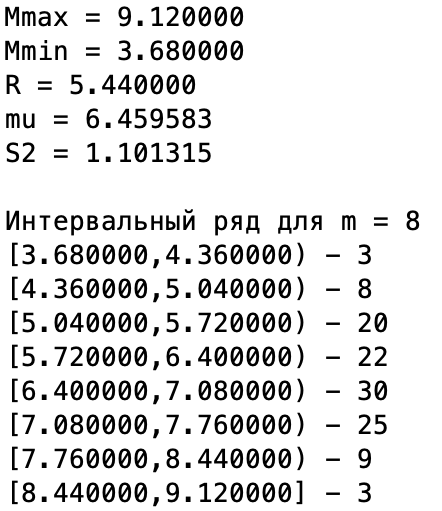
\includegraphics{values}

\item Гистограмма и график функции плотности распределения вероятностей нормальной случайной величины с математическим ожиданием $\hat \mu$ и дисперсией $S^2$. 

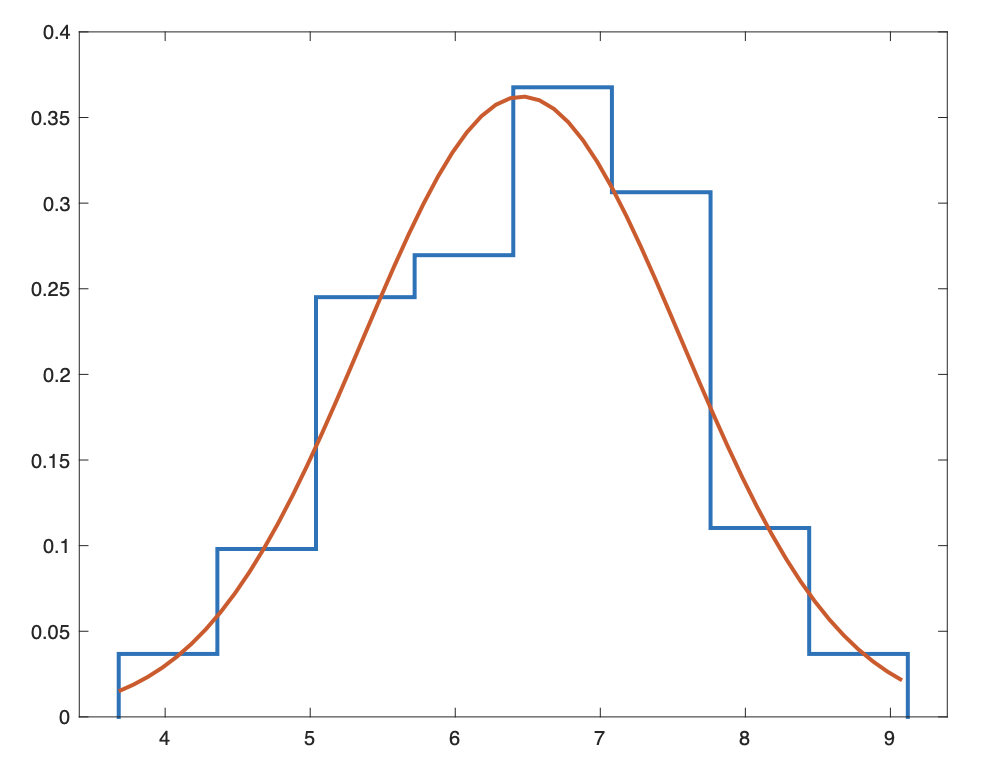
\includegraphics{graph1}

\newpage

\item График эмпирической функции распределения и функции распределения нормальной случайной величины с математическим ожиданием $\hat \mu$ и дисперсией $S^2$. 

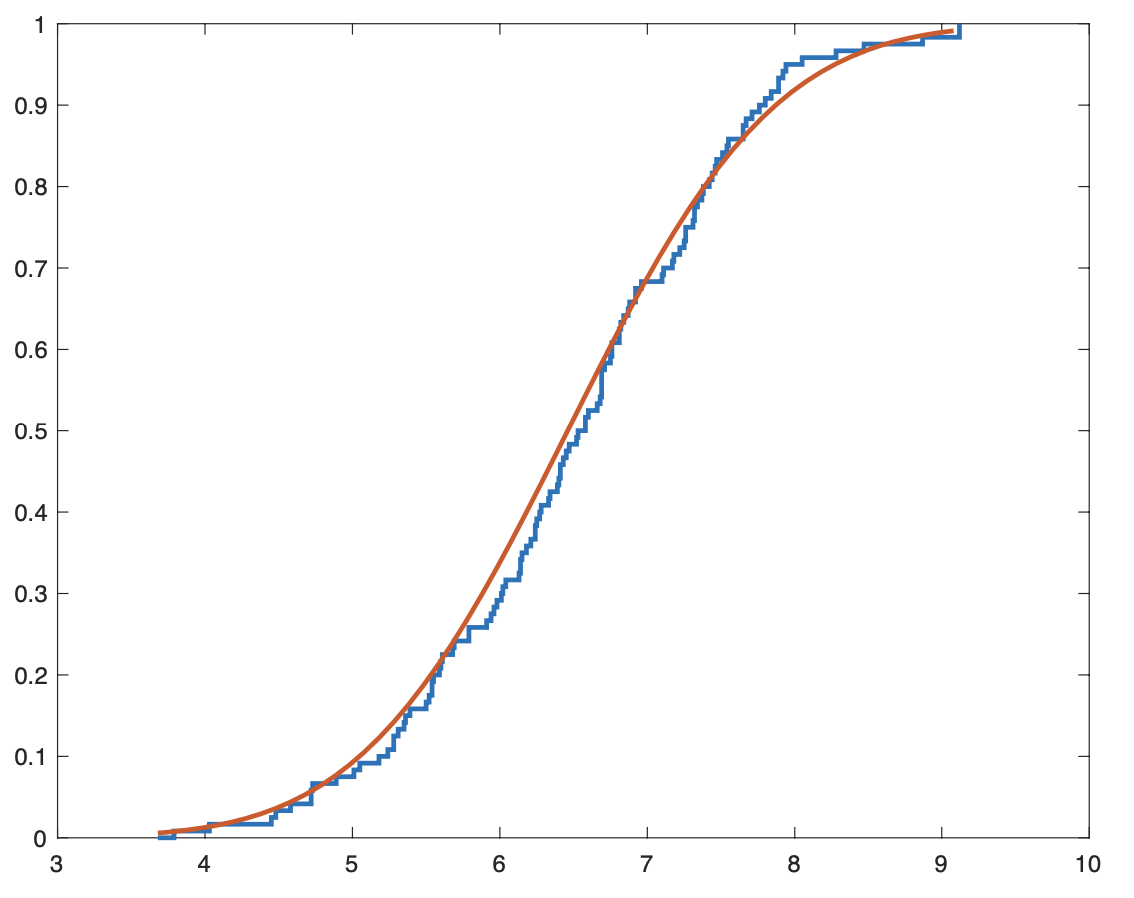
\includegraphics[scale=0.9]{graph2}

\end{enumerate}
\end{document}